\begin{refsection}[fs2020/ishikawa/group.bib]
\nocite{*}
\chapter{Flagship 2020 Project}

%%%%%%%%%%%%%%%%%%%%%%%%%%%%%%%%%%%%%%%%%%%%%%%%%%%%%%%%%%%%%%%%%%%%%%%%%%%%%
\section{Project Overview}
%%%%%%%%%%%%%%%%%%%%%%%%%%%%%%%%%%%%%%%%%%%%%%%%%%%%%%%%%%%%%%%%%%%%%%%%%%%%%
The Japanese government launched the FLAGPSHIP 2020 project
\footnote{ FLAGSHIP is an acronym for Future LAtency core-based
  General-purpose Supercomputer with HIgh Productivity.}
in JFYI 2014 whose missions are defined as follows:
\begin{itemize}
\item Building the Japanese national flagship supercomputer, the
  successor to the K computer, which is tentatively named the post K
  computer, and
\item developing wide range of HPC applications that will run on the
  post K computer in order to solve the pressing societal and
  scientific issues facing our country.
\end{itemize}

%%%
RIKEN accepted a request by the Ministry of Education, Culture,
Sports, Science and Technology (MEXT) to assume the responsibility of
being the institution responsible for the research and development of
the post K computer.
In the summer of 2014, the Japanese Government selected nine Priority
Issues to be targeted by the post K computer, and formulated project
organizations that would be responsible for research toward solving
them.  The government also selected four research areas which are named
Exploratory Challenging Issues to be developed.
Table \localref{tab:priority} lists the nine Priority Issues to be
tackled by the FLAGSHIP 2020 project and institutions selected to
lead the research for solving them.
Table \localref{tab:challenging} lists
four Exploratory Challenging Issues and selected institutions.

RIKEN AICS is in charge of co-design of the post K computer and
development of application codes in collaboration with the Priority
Issue institutes, as well as research aimed at facilitating the
efficient utilization of the post K computer by a broad community of
users.  Under the co-design concept, AICS and the selected
institutions are expected to collaborate closely.
For the post K computer system development, in September 2015, Fujitsu
Ltd. was selected to produce the basic design.
A number of university partners are partially involved with the design.

%%also collaborating with theeffort.
%%%

\begin{table}
\caption{Priority Issues}\locallabel{tab:priority}
\begin{center}
%\small
\footnotesize
\begin{tabular}{p{2cm}|p{5.2cm}|p{5.8cm}} \hline
\multirow{2}{*}{\vbox{Health and longevity}}
& 1. Innovative computing infrastructure for drug discovery
&	RIKEN Quantitative Biology Center, and other institutions \\ \cline{2-3}
& 2. Personalized and preventive medicine using big data
&	Institute of Medical Science / the University of Tokyo, and five other institutions \\ \hline
\multirow{2}{*}{\vbox{Disaster prevention / Environment}}
& 3. Integrated simulation systems induced by earthquake and tsunami Earthquake
&        Research Institute, the University of Tokyo and 4 other institutions \\ \cline{2-3}
& 4. Meteorological and global environmental prediction using big data
&	JAMSTEC / Center for Earth Information Science and Technology of Japan, and three other institutions\\ \hline
\multirow{2}{*}{\vbox{Energy issues}}
& 5. New technologies for energy creation, conversion / storage, and use
&	Institute for Molecular Science / National Institute of Neural Science, and eight other institutions \\ \cline{2-3}
& 6. Accelerated development of innovative clean energy systems
&	School of Engineering / the University of Tokyo, and eight other institutions\\ \hline
\multirow{2}{*}{\vbox{Industrial competitiveness enhancement}}
& 7. Creation of new functional devices and high-performance materials
&	The Institute of Solid State Physics / the University of Tokyo, and eight other institutions\\ \cline{2-3}
& 8. Development of innovative design and production processes
&	Institute of Industrial Science / the University of Tokyo, and six other institutions\\ \hline
Basic science
& 9. Elucidation of the fundamental laws and evolution of the universe
&	Center for Computational Science / Tsukuba University, and seven other institutions \\ \hline
\end{tabular}
\end{center}
\end{table}

\begin{table}
\caption{Exploratory Challenges}\locallabel{tab:challenging}
\begin{center}
%\small
\footnotesize
\begin{tabular}{p{6.2cm}|p{6.8cm}} \hline
\multirow{3}{*}{\vbox{10. Frontiers of basic science - challenge to the limits -}}
&       Institute for Material Research / Tohoku University, and nine other institutions \\ \cline{2-2}
&	Tokyo Woman's Christian University, and three other institutions \\ \cline{2-2}
&	School of Engineering / the University of Tokyo \\ \hline
\multirow{2}{*}{\vbox{11. Construction of models for interaction among multiple socioeconomic}}
&	RIKEN, Advanced Institute for Computational Science and twelve other institutions\\ \cline{2-2}
&	Tokyo University of Science and three other institutions\\ \hline
12. Elucidation of the birth of exoplanets (Second Earths) and the environmental variations of planets in the solar system
&	Kobe University Graduate School of Science and eight other institutions\\ \hline
\multirow{2}{*}{\vbox{13. Elucidation of how neural networks realize thinking and its application to artificial intelligence}}
&	Okinawa Institute of Science and Technology Graduate University and 4 other institutions\\ \cline{2-2}
&	The Research Center for Advanced Science and Technology / the University of Tokyo \\ \hline
\end{tabular}
\end{center}
\end{table}

%%%%%%%%%%%%%%%%%%%%%%%%%%%%%%%%%%%%%%%%%%%%%%%%%%%%%%%%%%%%%%%%%%%%%%%%%%%%%
\section{AICS Teams}
%%%%%%%%%%%%%%%%%%%%%%%%%%%%%%%%%%%%%%%%%%%%%%%%%%%%%%%%%%%%%%%%%%%%%%%%%%%%%
As shown in Table \localref{tab:aicsorg}, four development teams are
working on post K computer system development with the FLAGSHIP 2020
Planning and Coordination Office that supports development activities.
The primary members are listed in Section \localref{sec:members}.
 
\begin{table}
\caption{Development Teams}\locallabel{tab:aicsorg}
\begin{center}
\footnotesize
\begin{tabular}{c|c|c} \hline
Team Name & Team Leader & Number of Members\\ \hline
Architecture Development &	Mitsuhisa Sato  & XX\\
System Software Development &	Yutaka Ishikawa & XX \\
Co-Design &	Junichiro Makino\\ \hline
Application Development &	Hirofumi Tomita & XX\\
\end{tabular}
\end{center}
\end{table}

%
% Sato
The Architecture Development team designs the architecture of the post
K computer in cooperation with Fujitsu and designs and develops a
productive programming language, called XcalableMP (XMP), and its
tuning tools.
The team also specifies requirements of standard languages such as Fortran
and C/C++ and mathematical libraries provided by Fujitsu.

The System Software Development team designs and specifies a system
software stack such as Linux, MPI and File I/O middleware for the post
K computer in cooperation with Fujitsu and designs and develops
multi-kernel for manycore architectures, Linux with light-weight
kernel (McKernel), that provides a noise-less runtime environment,
extendability and adaptability for future application demands.  The
team also designs and develops a low-level communication layer to
provide scalable, efficient and portability for runtime libraries and
applications.

%
% Makino
The Co-Design team leads to optimize architectural features and
application codes together in cooperation with AICS teams and Fujitsu.
It also designs and develops an application framework,
FDPS (Framework for Developing Particle Simulator),
to help HPC users implement advanced algorithms.

%
% Tomita
The Application Development team is a representative of nine institutions
aimed at solving Priority Issues.
The team figures out weakness of target application codes in terms of
performance and utilization of hardware resources and discusses
them with AICS teams and Fujitsu to find out best solutions of
architectural features and improvement of application codes.

%%%%%%%%%%%%%%%%%%%%%%%%%%%%%%%%%%%%%%%%%%%%%%%%%%%%%%%%%%%%%%%%%%%%%%%%%%%%
\section{Co-design with applications from Priority Issues}
%%%%%%%%%%%%%%%%%%%%%%%%%%%%%%%%%%%%%%%%%%%%%%%%%%%%%%%%%%%%%%%%%%%%%%%%%%%%
During the development stage, emphasis will be placed on co-design
concepts that allow the system and application development processes
to work harmoniously together so that the societal and scientific
issues can be solved effectively and early achievements can be
attained.  Since increasing power consumption is a critical issue in
the design of the next-generation large-scale supercomputer, it will
be important for the co-design to make trade-offs between
energy/power, cost, and performance by taking application
characteristics into consideration.
It should be noted that we design the entire system using a
proprietary processor and interconnect, in collaboration with Fujitsu,
rather than choosing existing components to construct the system.

Table \localref{tab:targets} shows a set of target applications
provided from each area of the nine Priority Issues. System design is
being performed using these applications as a target in the co-design
process.

\begin{table}
\caption{Target Applications}\locallabel{tab:targets}
\begin{tabular}{p{24mm}|p{122mm}} \hline
Program & Brief Description \\ \hline
GENESIS & Molecular dynamics simulation for protein in solvent (MD) \\
Genomon & Human Genome processing (Genome alignment) \\
GAMERA  & Earthquake simulation system (FEM multigrid method)\\
NICAM+LETKF & Weather prediction system using Big data (structured grid \& ensemble Kalman filter)\\
NTChem  & Ab-initio molecular electronic structure (RI-MP2 method)\\
ADVENTURE &	Computational mechanics system for large scale analysis and design (unstructured grid) \\
RSDFT   & Ab-initio simulation based on density functional theory (real space DFT method)\\
FFB     & FEM flow analysis around the complex geometry (Large Eddy Simulation)\\
LQCD	& Lattice QCD simulation (structured grid Monte Carlo)\\ \hline
\end{tabular}
\end{table}

%\clearpage

\begin{figure}
\begin{center}
 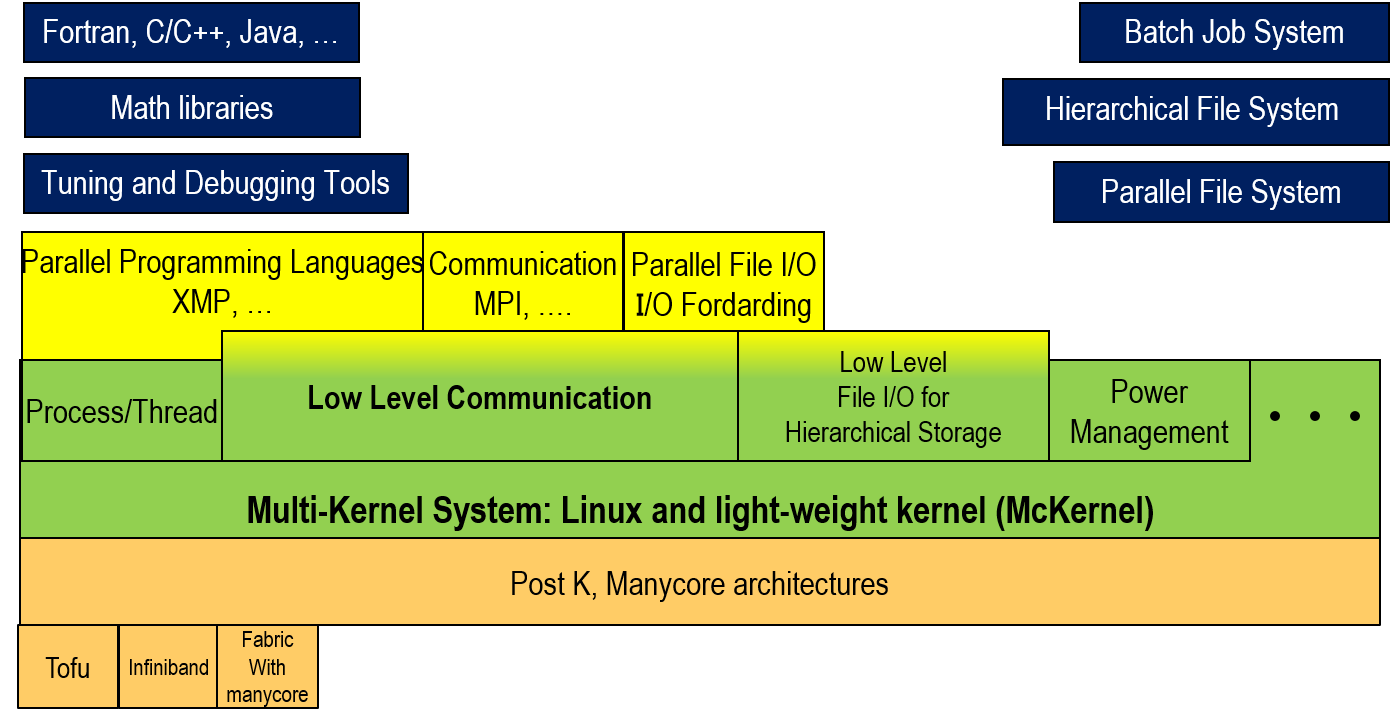
\includegraphics[width=0.9\textwidth,natwidth=1043,natheight=542]{softarch.png}
\end{center}
\caption{Software Architecture}\locallabel{fig:softarch}
\end{figure}

%%%%%%%%%%%%%%%%%%%%%%%%%%%%%%%%%%%%%%%%%%%%%%%%%%%%%%%%%%%%%%%%%%%%%%%%%%%%%
\section{Target of System Development and Basic Design}
%%%%%%%%%%%%%%%%%%%%%%%%%%%%%%%%%%%%%%%%%%%%%%%%%%%%%%%%%%%%%%%%%%%%%%%%%%%%%
The post K's design targets are as follows:
\begin{itemize}
\item A one hundred times speed improvement over the K computer is
  achieved in maximum case of some target applications. This will be
  accomplished through co-design of system development and target
  applications for the nine Priority Issues.
\item The maximum electric power consumption should be between 30 and
  40 MW.
\end{itemize}

In 2014, the basic design of the system was completed.  The AICS
decided to adopt a general-purpose many-core architecture rather than
using accelerators, such as graphics processing units (GPUs), in order
to support a wider range of applications.
At the time of writing, Fujitsu has just announced that the node
processor is based on an ARM architecture with Fujitsu HPC extensions
that was invented for the K computer.
To ensure the performance of large-scale parallel applications
remained compatible with the K computer, we choose a similar topology
for the interconnect, Tofu interconnect (6D mesh/torus).

The major components of system software shown in Figure \localref{fig:softarch}
have been decided to be developed.
These are summarized as follows:

\begin{itemize}
% Sato
\item Highly productive programming language, XcalableMP\\
XcalableMP (XMP) is a directive-based PGAS language for large scale
distributed memory systems that combines HPF-like concept and
OpenMP-like description with directives.
Two memory models are supported: global view and local view.  The
global view is supported by the PGAS feature, i.e., large array is
distributed to partial ones in nodes.  The local view is provided by
MPI-like + Coarray notation.

% Makino
\item Domain specific library/language, FDPS\\
FDPS is a framework for the development of massively parallel particle simulations.
Users only need to program particle interactions and do not
need to parallelize the code using the MPI library.
The FDPS adopts highly optimized communication algorithms and
its scalability has been confirmed using the K computer.

\item MPI + OpenMP programming environment\\
The current de facto standard programming environment,
i.e., MPI + OpenMP environment, is supported.
Two MPI implementations are being developed.
Fujitsu continues to support own MPI implementation based on the OpenMPI.
RIKEN is collaborating with ANL (Argonne National Laboratory) to develop
MPICH, mainly developed at ANL, for post K computer.

\item New file I/O middleware\\
The post K computer does not employ the file staging technology 
for the layered storage system.
The users do not need to specify which files must be staging-in and
staging-out in their job scripts in the post K computer environment.
Asynchronous I/O and caching technologies are fully utilized in the post
K computer in order to provide transparent file access with better performance.

\item Application-oriented file I/O middleware\\
In scientific Big-Data applications, such as real-time weather
prediction using observed meteorological data, a rapid data transfer
mechanism between two jobs, ensemble simulations and data
assimilation, is required to meet their deadlines.
Keeping a file I/O interface, such as netCDF, direct data transfer
between two jobs without involving a storage system is being designed
and implemented.

\item Multi-Kernel for manycore architectures\\
Multi-Kernel, Linux with light-weight Kernel (McKernel) is being
designed and implemented.
It provides:
i) a noiseless execution environment for bulk-synchronous applications,
ii) ability to easily adapt to new/future system architectures, e.g.,
manycore CPUs, a new process/thread management, a memory management,
heterogeneous core architectures, deep memory hierarchy, etc., and
iii) ability to adapt to new/future application demands, such as
Big-Data and in-situ applications that require optimization of data movement.
\end{itemize}
% Sato and Makino, do we need some more statements, e.g. GPGPU ?
It should be noted that these components are not only for post K computer,
but also for other manycore-based supercomputer, such as Intel Xeon Phi.

%%%%%%%%%%%%%%%%%%%%%%%%%%%%%%%%%%%%%%%%%%%%%%%%%%%%%%%%%%%%%%%%%%%%%%%%%%%%
\section{Schedule}
%%%%%%%%%%%%%%%%%%%%%%%%%%%%%%%%%%%%%%%%%%%%%%%%%%%%%%%%%%%%%%%%%%%%%%%%%%%%
At the time of writing, the new development plan has been announced by the
government.
As shown in Figure \localref{fig:schedule}, the design and prototype
implementations will be done before the end of 2019, and the system
will be deployed after this phase.  The service is expected to start
public operation at the range from 2021 to 2022.

\begin{figure}
\begin{center}
 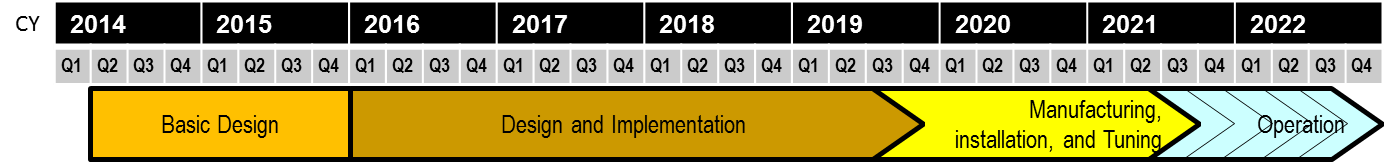
\includegraphics[width=0.9\textwidth,natwidth=1040,natheight=126]{flagship2020-schedule.png}
\end{center}
\caption{Schedule}\locallabel{fig:schedule}
\end{figure}

%%%%%%%%%%%%%%%%%%%%%%%%%%%%%%%%%%%%%%%%%%%%%%%%%%%%%%%%%%%%%%%%%%%%%%%%%%%%
\section{Members}\locallabel{sec:members}
%%%%%%%%%%%%%%%%%%%%%%%%%%%%%%%%%%%%%%%%%%%%%%%%%%%%%%%%%%%%%%%%%%%%%%%%%%%%
Primary members are only listed.

%===========================================================================
\subsection{System Software Development Team}
%===========================================================================
\begin{itemize}
  \item[] Yutaka Ishikawa (Team Leader)
  \item[] Masamichi Takagi (Senior Scientist)
  \item[] Atsushi Hori	(Research Scientist)
  \item[] Balazs Gerofi	(Research Scientist)
  \item[] Masayuki Hatanaka	(Research \& Development Scientist)
  \item[] Takahiro Ogura	(Research \& Development Scientist)
  \item[] Tatiana Martsinkevich	(Postdoctoral Researcher)
  \item[] Fumiyoshi Shoji	Research \& Development Scientist
  \item[] Atsuya Uno	Research \& Development Scientist
  \item[] Toshiyuki Tsukamoto	Research \& Development Scientist
\end{itemize}

%===========================================================================
\subsection{Architecture Development}
%===========================================================================
% Sato, needs more member ?
\begin{itemize}
  \item[] Mitsuhisa Sato (Team Leader)
  \item[] Yuetsu Kodama	(Senior Scientist)
  \item[] Miwako Tsuji	(Research Scientist)
  \item[] Hidetoshi Iwashita	(Research \& Development Scientist)
  \item[] Jinpil Lee	(Postdoctoral Researcher)
  \item[] Tetsuya Odajima	(Postdoctoral Researcher)
  \item[] Hitoshi Murai	(Research Scientist)
  \item[] Toshiyuki Imamura	(Research Scientist)
\end{itemize}

%===========================================================================
\subsection{Application Development}
%===========================================================================
% Tomita, needs more member ?
\begin{itemize}
  \item[] Hirofumi Tomita (Team Leader)
  \item[] Yoshifumi Nakamura	(Research Scientist)
  \item[] Hisashi Yashiro	(Research Scientist)
  \item[] Seiya Nishizawa	(Research Scientist)
  \item[] Hiroshi Ueda	Research (Scientist)
  \item[] Yukio Kawashima	(Research Scientist)
  \item[] Naoki Yoshioka	(Research Scientist)
  \item[] Yiyu Tan	(Research Scientist)
  \item[] Soichiro Suzuki	Research \& Development Scientist
  \item[] Kazunori Mikami	Research \& Development Scientist
\end{itemize}

%===========================================================================
\subsection{Co-Design}
%===========================================================================
% Makino, needs more member ?
\begin{itemize}
  \item[] Junichiro Makino (Team Leader)
  \item[] Keigo Nitadori	(Research Scientist)
  \item[] Yutaka Maruyama	(Research Scientist)
%  \item[] Mikio Iizuka	Research (Scientist)
  \item[] Takayuki Muranushi	(Postdoctoral Researcher)
\end{itemize}

%%% DO NOT EDIT BELOW

\section{Publications}

%\printbibliography[keyword=journal, heading=subbibliography, title={Journal Articles}, prefixnumbers={1-}, resetnumbers=true]
%\printbibliography[keyword=proceedings, heading=subbibliography, title={Conference Papers}, prefixnumbers={2-}, resetnumbers=true]
%\printbibliography[keyword=invited, heading=subbibliography, title={Invited Talks}, prefixnumbers={3-}, resetnumbers=true]
%\printbibliography[keyword=poster, heading=subbibliography, title={Posters and Presentations}, prefixnumbers={4-}, resetnumbers=true]
%\printbibliography[keyword=deliverable, heading=subbibliography, title={Patents and Deliverables}, prefixnumbers={5-}, resetnumbers=true]

\printbibliography[keyword=journal, heading=subbibliography, title={Journal Articles}, resetnumbers=true]
\printbibliography[keyword=proceedings, heading=subbibliography, title={Conference Papers}]
\printbibliography[keyword=invited, heading=subbibliography, title={Invited Talks}]
\printbibliography[keyword=poster, heading=subbibliography, title={Posters and Presentations}]
\printbibliography[keyword=deliverable, heading=subbibliography, title={Patents and Deliverables}]

\end{refsection}
